
%%%%%%%%%%%%%%%%%%%%%%%%%%%%%%%%%%%%%%%%%
% Structured General Purpose Assignment
% LaTeX Template
%
% This template has been downloaded from:
% http://www.latextemplates.com
%
% Original author:
% Ted Pavlic (http://www.tedpavlic.com)
%
% Note:
% The \lipsum[#] commands throughout this template generate dummy text
% to fill the template out. These commands should all be removed when 
% writing assignment content.
%
%%%%%%%%%%%%%%%%%%%%%%%%%%%%%%%%%%%%%%%%%

%----------------------------------------------------------------------------------------
%	PACKAGES AND OTHER DOCUMENT CONFIGURATIONS
%----------------------------------------------------------------------------------------

\documentclass{article}

\usepackage{fancyhdr} % Required for custom headers
\usepackage{lastpage} % Required to determine the last page for the footer
\usepackage{extramarks} % Required for headers and footers
\usepackage{graphicx} % Required to insert images
\usepackage{lipsum} % Used for inserting dummy 'Lorem ipsum' text into the template

% Margins
\topmargin=-0.45in
\evensidemargin=0in
\oddsidemargin=0in
\textwidth=6.5in
\textheight=9.0in
\headsep=0.25in 

\linespread{1.1} % Line spacing
\pdfinfo{
   /Author (Sainyam Kapoor)
   /Title  (Assignment)
   /CreationDate (D:20140115195600)
   /Subject (Assignment1)
   /Keywords (PDF;assignment CS-2204)
}
% Set up the header and footer
\pagestyle{fancy}
\lhead{\hmwkAuthorName} % Top left header
\chead{\hmwkClass\ (\hmwkClassInstructor\ ): \hmwkTitle} % Top center header
\rhead{\firstxmark} % Top right header
\lfoot{\lastxmark} % Bottom left footer
\cfoot{} % Bottom center footer
\rfoot{Page\ \thepage\ of\ \pageref{LastPage}} % Bottom right footer
\renewcommand\headrulewidth{0.4pt} % Size of the header rule
\renewcommand\footrulewidth{0.4pt} % Size of the footer rule

\setlength\parindent{0pt} % Removes all indentation from paragraphs

%----------------------------------------------------------------------------------------
%	DOCUMENT STRUCTURE COMMANDS
%	Skip this unless you know what you're doing
%----------------------------------------------------------------------------------------

% Header and footer for when a page split occurs within a problem environment
\newcommand{\enterProblemHeader}[1]{
\nobreak\extramarks{#1}{#1 continued on next page\ldots}\nobreak
\nobreak\extramarks{#1 (continued)}{#1 continued on next page\ldots}\nobreak
}

% Header and footer for when a page split occurs between problem environments
\newcommand{\exitProblemHeader}[1]{
\nobreak\extramarks{#1 (continued)}{#1 continued on next page\ldots}\nobreak
\nobreak\extramarks{#1}{}\nobreak
}

\setcounter{secnumdepth}{0} % Removes default section numbers
\newcounter{homeworkProblemCounter} % Creates a counter to keep track of the number of problems

\newcommand{\homeworkProblemName}{}
\newenvironment{homeworkProblem}[1][Problem \arabic{homeworkProblemCounter}]{ % Makes a new environment called homeworkProblem which takes 1 argument (custom name) but the default is "Problem #"
\stepcounter{homeworkProblemCounter} % Increase counter for number of problems
\renewcommand{\homeworkProblemName}{#1} % Assign \homeworkProblemName the name of the problem
\section{\homeworkProblemName} % Make a section in the document with the custom problem count
\enterProblemHeader{\homeworkProblemName} % Header and footer within the environment
}{
\exitProblemHeader{\homeworkProblemName} % Header and footer after the environment
}

\newcommand{\problemAnswer}[1]{ % Defines the problem answer command with the content as the only argument
\noindent\framebox[\columnwidth][c]{\begin{minipage}{0.98\columnwidth}#1\end{minipage}} % Makes the box around the problem answer and puts the content inside
}

\newcommand{\homeworkSectionName}{}
\newenvironment{homeworkSection}[1]{ % New environment for sections within homework problems, takes 1 argument - the name of the section
\renewcommand{\homeworkSectionName}{#1} % Assign \homeworkSectionName to the name of the section from the environment argument
\subsection{\homeworkSectionName} % Make a subsection with the custom name of the subsection
\enterProblemHeader{\homeworkProblemName\ [\homeworkSectionName]} % Header and footer within the environment
}{
\enterProblemHeader{\homeworkProblemName} % Header and footer after the environment
}
   
%----------------------------------------------------------------------------------------
%	NAME AND CLASS SECTION
%----------------------------------------------------------------------------------------

\newcommand{\hmwkTitle}{Assignment\ \#1} % Assignment title
\newcommand{\hmwkDueDate}{Sunday,\ January\ 19,\ 2014} % Due date
\newcommand{\hmwkClass}{CS-2204} 
\newcommand{\hmwkClassName}{DESIGN AND ANALYSIS OF ALGORITHMS} % Course/class

\newcommand{\hmwkClassInstructor}{Dr. Ravi Shankar Singh} % Teacher/lecturer
\newcommand{\hmwkAuthorName}{Sainyam Kapoor} % Your name

%----------------------------------------------------------------------------------------
%	TITLE PAGE
%----------------------------------------------------------------------------------------

\title{
\vspace{2in}
\textmd{\textbf{\hmwkClass:\ \hmwkTitle\\~\\ \hmwkClassName}}\\
\normalsize\vspace{0.1in}\small{Due\ on\ \hmwkDueDate}\\
\vspace{0.1in}\large{\textit{Submitted to \hmwkClassInstructor\ }}
\vspace{2in}
\vspace{0.1in}\large{\textit{\\~\\Submitted by }}}

\author
 {
\textbf{\hmwkAuthorName}
\\~\\
\textit{12400EN003}
}

\date{17 January 2014} % Insert date here if you want it to appear below your name

%----------------------------------------------------------------------------------------

\begin{document}

\maketitle

\clearpage

%----------------------------------------------------------------------------------------
%	PROBLEM 1
%----------------------------------------------------------------------------------------

% To have just one problem per page, simply put a \clearpage after each problem

\begin{homeworkProblem}
\textbf{How many times F(n-i) is called in recursive computation of F(n)?} \vspace{10pt} % Question

\problemAnswer{ 
\begin{center}
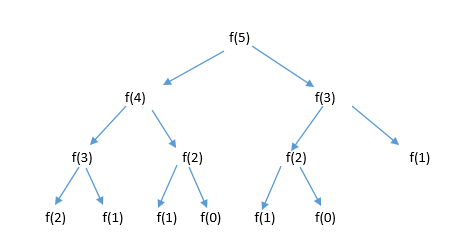
\includegraphics[width=0.75\columnwidth]{q1} % Example image
\end{center}
Observing the above tree it can be easily concluded that f(n) appears as many times as the sum the number of times f(n+1) and f(n+2) appears in the sum. \\~\\
Let T(i) represent the function that shows the number of times f(i) appears in calculation of f(n) 
\\~\\Clearly ,
T(n+1) = 0 = f(0)\\~\\ 
T(n) = 1 = f(1)\\~\\ 
T(n-1) = 1 = f(2)\\~\\ 

. \\~\\

We observe that T(n-i) = f(i+1) where f(i) represents the Fibonacci series. 
\\~\\Hence ans is f(i+1) 
\\~\\f(n) = f(n-1) + f(n-2) 
\\~\\Solving this recurrence (x$^{2}$= x + 1 ) we get  
\\~\\r$_{1}$ = (1+$\sqrt{5}$)/2 
\\~\\r$_{2}$ = (1-$\sqrt{5}$)/2  
\\~\\Therefore f(n) = C$_{1}$(r$_{1}$)$^{n}$ + C$_{2}$(r$_{2}$)$^{n}$
\\~\\Here C$_{1}$ = 1/$\sqrt{5}$ and C$_{2}$ = -1 /$\sqrt{5}$ }
\end{homeworkProblem}

%----------------------------------------------------------------------------------------
%	PROBLEM 1
%----------------------------------------------------------------------------------------

% To have just one problem per page, simply put a \clearpage after each problem
\clearpage
\begin{homeworkProblem}
\textbf{Compare the two functions n**2 and 2**(n)/4 for various values of n by making the plot. Determine when the second becomes larger than the first.}  \vspace{10pt} % Question

\problemAnswer{ 

\begin{center}
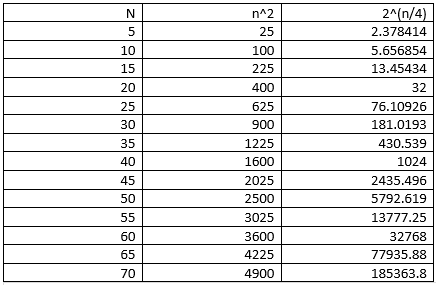
\includegraphics[width=0.75\columnwidth]{q2} 
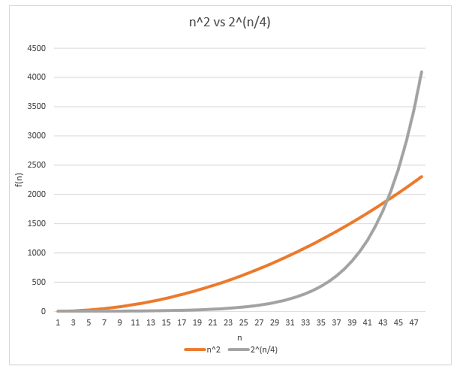
\includegraphics[width=0.75\columnwidth]{q2_2}% Example image
\end{center}
The Graph Intersects at 43.55.
}
\end{homeworkProblem}


% To have just one problem per page, simply put a \clearpage after each problem
\clearpage
\begin{homeworkProblem}
\textbf{Is 2$^{2n}$ = O(2$^{n}$)?}  \vspace{10pt} % Question

\problemAnswer{ 

By definition of O notation f(x) = O(g(x)) iff 
\\~\\ 
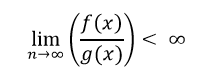
\includegraphics{q3} 
\\~\\ Applying  the above equations we get 
\\~\\ 
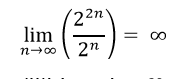
\includegraphics{q4} 
\\~\\ Thus 2$^{2n}$ is not equal to O(2$^{n}$).

}
\end{homeworkProblem}
\end{document}
